% o \label{codigo} serve para podermos fazer referencias para algo numerado, 
% como capitulos, tabelas, figuras, etc. 
% Quando colocamos o comando \ref{codigo}. o compilador troca o \ref{codigo}
% pelo numero atribuido ao \label{}
% ex. \label{tabelaLegal}
%   A tabela \ref{tabelaLegal} mostra que...
% vai ser substituido por
%   A tabela 2 mostra que

\chapter{Desenvolvimento}\label{cap-desenvolvimento}

Segundo o processo iterativo de desenvolvimento descrito na metodologia, este projeto evoluiu ao longo de várias etapas de crescente complexidade.


% ---
\section{Objetivo e formulação do problema}\label{sec-objetivos-formulacao-problema}
% ---

Foi inicialmente elaborada uma enunciação geral do problema a ser resolvido: a criação de um jogo digital que, valendo-se de técnicas de realidade virtual, oferecesse uma experiência imersiva e educativa a crianças de 8 a 12 anos de idade, de acordo com o recorte selecionado descrito da seção \ref{cap-teoria} de **Teoria**. Tendo essa enunciação como base, pôde-se decidir a respeito de restrições, e do escopo que guiariam as etapas seguintes de conceituação do projeto.

% ---
\subsection{Delimitação do escopo}\label{subsec-delimitacao-escopo}
% ---
TODO

% ---
\subsection{Recorte do público alvo}\label{subsec-recorte-publico-alvo}
% ---

Em primeiro lugar, optou-se por restringir os equipamentos e tecnologias a serem empregados, de modo a facilitar a acessibilidade e adoção em sala de aula e diminuir os custos implantação, sem que a experiência desejada tivesse de ser sacrificada. Isso levou à escolha do uso do Google Cardboard como dispositivo principal de realidade virtual, por seu baixo custo comparado a demais alternativas de mercado, e sua integração a dispositivos móveis que, em muitos casos, já estariam ao alcance dos alunos, ou poderiam ser providenciados sem um grande impacto orçamentário.

Em adição ao Cardboard, optou-se pela implemntação do dispositivo detector de gestos manuais Leap Motion como forma de *input* principal para o jogo, com a vantagem de ser uma alternativa de custo aceitável, capaz de providenciar uma experiência bastante direta na interação do aluno com o mundo do jogo, uma vez que permite que movimentos do jogador no mundo real sejam traduzidos em ações do mundo virtual, permitindo abstrair oos dispositivos de entrada e saída por completo, e mantendo a imersão e engajamento.

Por fim, como restrição adicional, a ferramenta Unity foi escolhida como *engine* de desenvolvimento do jogo, por sua fácil integração ao hardware escolhido, e seu paradigma de desenvolvimento em mais alto nível do que as demais alternativas disponíveis, o que permitiria ao grupo focar-se na conceituação e implementação do jogo em si, sem prender-se a eventuais problemas relativos à configuração e uso do hardware, criação de APIs próprias ou preocupações com elementos mais elementares da criação de um jogo digital.

% ---
\section{Brainstorming e seleção do conceito do jogo}\label{sec-brainstorming-conceito}
% ---

Com a enunciação do problema e as restrições de implementação bem definidas e acordadas pelo grupo, pôde-se passar para a etapa seguinte do desenvolvimento, o *brainstorm*, durante o qual várias ideias foram debatidas e exploradas pelos membros do grupo. Nesta fase, diversas propostas foram feitas para uma solução que fizesse um bom uso dos recursos de realidade virtuais disponíveis e gerasse um projeto adequado ao público alvo selecionado, resultando em um jogo intuitivo, divertido que capaz de transmitir os conceitos de lógicos e cognitivos relevantes.

As ideias geradas variaram desde jogos de um ritmo mais acelerado, no qual um jogador teria que categorizar elementos abstratos o mais rápido que pudesse - segundo características como cor, formato e tamanho - até experiências nas quais pressões de tempo e condições de falha estavam copletamente ausentes, como jogos de resolução de quebra-cabeças tridimensionais.

\begin{figure}[h]
	\centering
	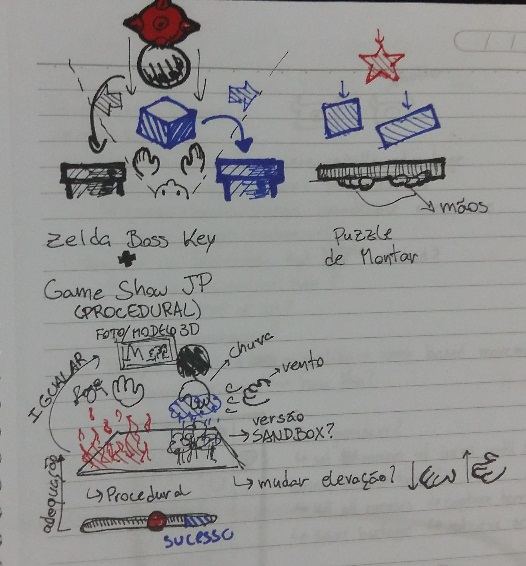
\includegraphics[width=0.5\textwidth]{first_concepts}
	\caption{primeiro rascunho do jogo}
\end{figure}

Por fim, uma análise cuidadosa das limitações das tecnologias escolhidas, aliada a uma preocupação em manter o jogo intuitivo e imersivo levaram o grupo a um design mais diretamente análogo ao mundo real, gerando um jogo no qual o jogador manipularia características de uma pequena configuração geológica tridimensional, de forma a manipulá-la para chegar a um determinado estado pré-definido.

Neste jogo, as crianças se deparariam com um terreno digital composto por acidentes geográficos como planaltos, depressões, corpos d'água e formações magmáticas, e poderiam modificá-lo a partir de gestos manuais simples que controlassem a elevação, precipitação, movimentação do ar, entre outros. Este terreno seria subdivido em unidades cúbicas que poderiam ser manipuladas individualmente, fornecendo uma resolução suficiente para que configurações diversas e interessantes pudessem ser construídas, mas sem exigir uma precisão incompatível com os dispositivos de entrada e saída escolhidos.

\begin{figure}[h]
	\centering
	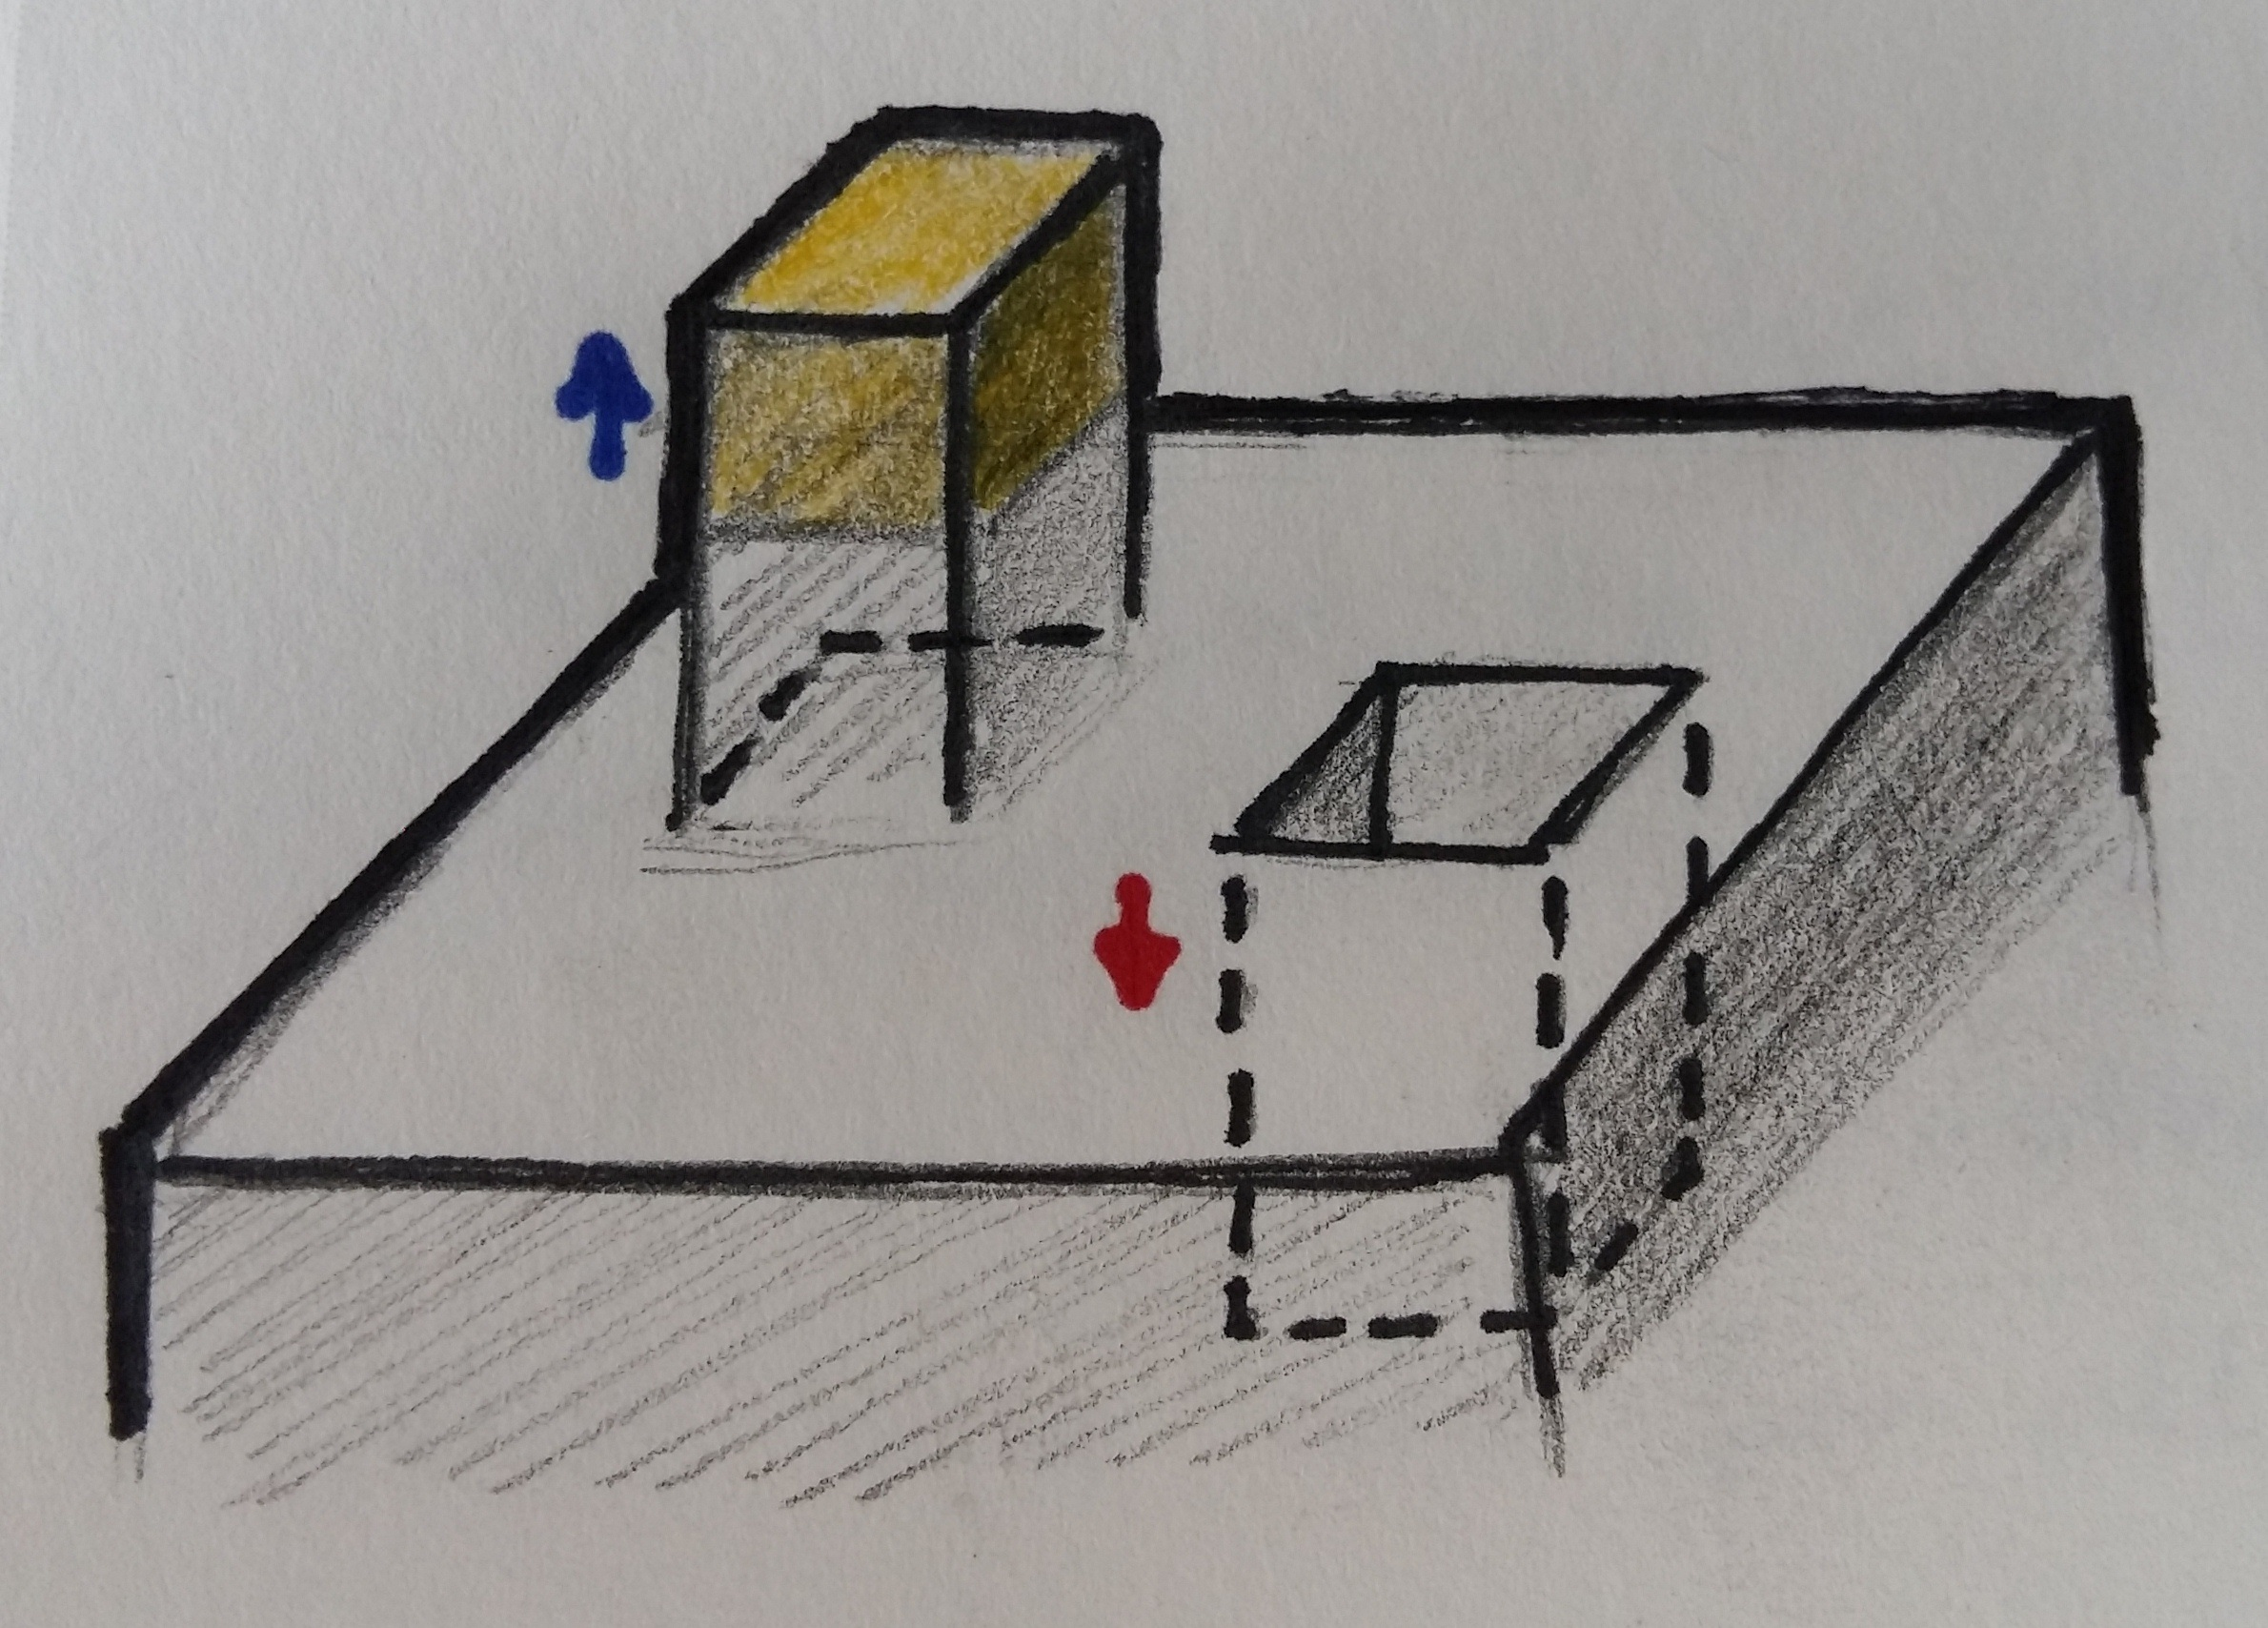
\includegraphics[width=0.5\textwidth]{draft1}
	\caption{Conceitos iniciais}
\end{figure}


Foram então imaginados cenários que extrapolassem os usoss básicos das mecânicas propostas, de maneiras que se alinhassem aos conceitos pedagógicos que que deveriam ser transmitidos pelo jogo: desafios que dependessem da execução de tarefas em uma determinada ordem, em combinação com outras tarefas paralelas, ou dentro de um determinado limite de tempo. Nestes cenários, era esperado que jogadores conseguissem imaginar soluções mais sofisticadas, indo além das interações básicas às quais teriam acesso direto. Seria necessário movimentar massas de ar para jogar água contra blocos de terra, formando praias; escavar o solo para alcançar câmaras magmáticos e formar vulcões; ou alterar o curso de corpos d'água para formar cascatas.

\begin{figure}[htb]
	\centering
	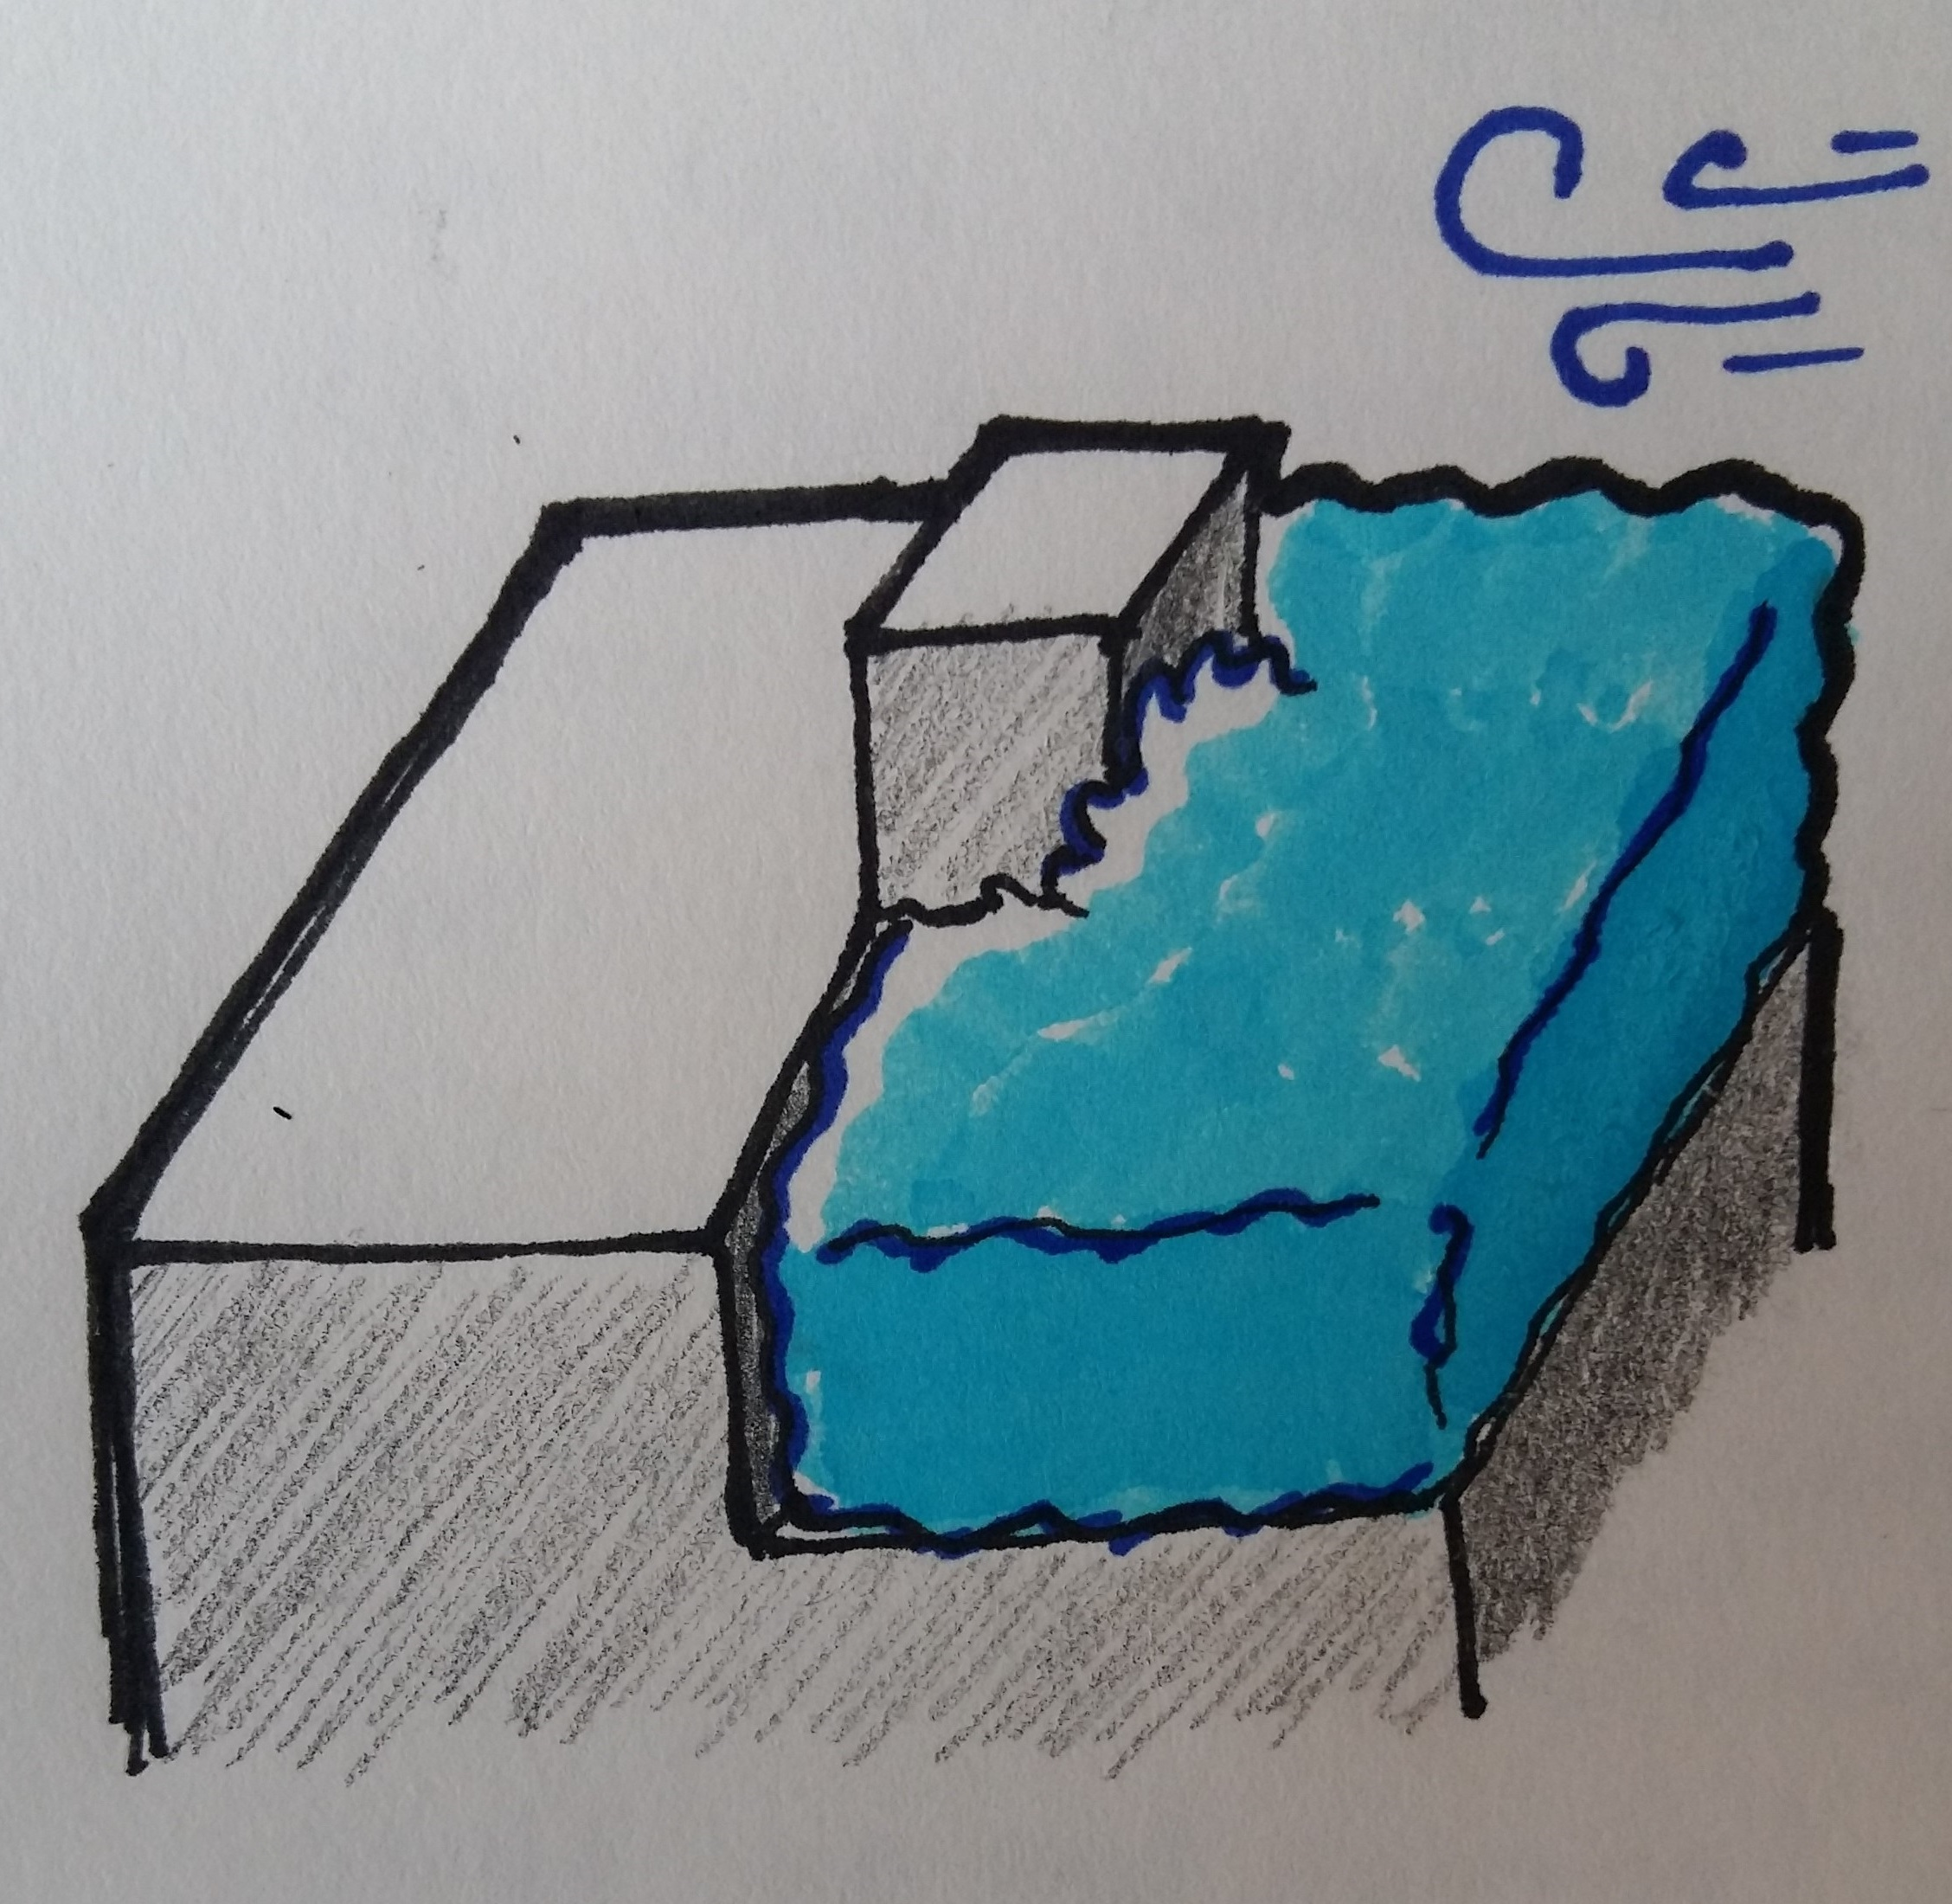
\includegraphics[width=0.5\textwidth]{draft2}
	\caption{Primeiro rascunho do jogo}
\end{figure}

% ---
\section{Primeira iteração: prova de conceito}\label{sec-primeira-iteracao-prova-conceito}
% ---

Uma vez decidido o conceito a ser explorado, um pequeno protótipo foi proposto para dar ao grupo uma noção mais palpável de como esse jogo se pareceria, como seria controlá-lo, que dificuldades imprevistas apareceriam e quais as medidas que precisariam ser tomadas para suplantá-las. Este protótipo inicial tinha como objetivo tanto familiarizar o grupo às ferramentas e tecnologias escolhidas para a realização do trabalho quando ajudar a nivelar de maneira mais concreta a complexidade de sua implementação.

O protótipo deveria se ater apenas a uma mecânica básica da especificação do conceito: controle da elevação do terreno. O jogador teria acesso direto ao jogo - sem passar por telas de menu ou tutoriais - no qual se depararia com uma grade tridimensional de 5x5x5 cubos de terra, os quais poderia elevar ou rebaixar livremente.

\begin{figure}[h]
	\centering
	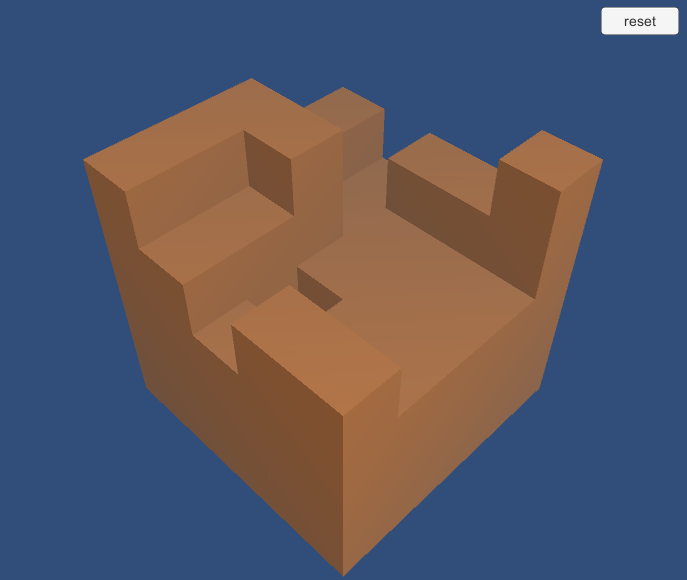
\includegraphics[width=0.5\textwidth]{ss1}
	\caption{Prova de conceito do jogo}
\end{figure}

Apesar da simples implementação, algumas  primeiras dificuldades já puderam ser percebidas nesta iteração, sobretudo na integração dos dispositivos de realidade virtual.

A primeira barreira a ser percebida foi a falta de compatibilidade com dispositivos Android da versão mais recente do SDK do controlador Leap Motion, como havia nas versões anteriores. Isso, aliado ao fato de que a versão anterior do SDK não estava mais disponível para download, significou que uma interação direta entre o Leap Motion e o jogo compilado para dispositivos móveis não seria possível nessa etapa inicial do projeto.

Apesar deste empecilho, Unity se mostrou uma plataforma robusta e flexível o suficiente para a continuação do projeto, e as mecânicas básicas puderam ser implementadas rapidamente e sem grandes problemas.

% ---
\section{Segunda iteração: mecânicas básicas}\label{sec-segunda-iteracao-mecanicas-basicas}
% ---

Tendo em mente as facilidades e desafios percebidos durante a criação da prova de conceito, um segundo protótipo foi desenvolvido, desta vez com o intuito de acrescentar uma segunda mecânica básica - controle da precipitação - de modo a permitir que o jogador experimentasse com a interação entre as duas.

\begin{figure}[ht]
	\centering
	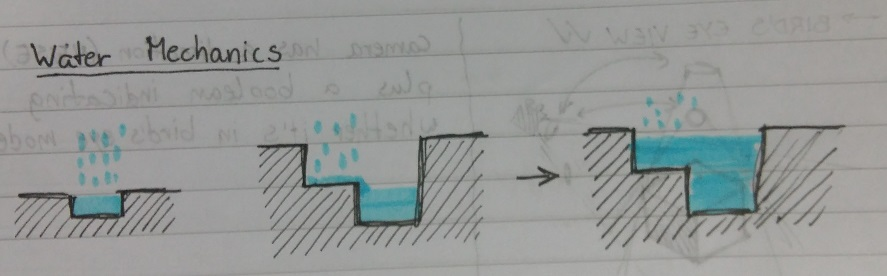
\includegraphics[width=0.5\textwidth]{water_mechanics1}
	\caption{Mecânicas da água 1}
\end{figure}

\begin{figure}[ht]
	\centering
	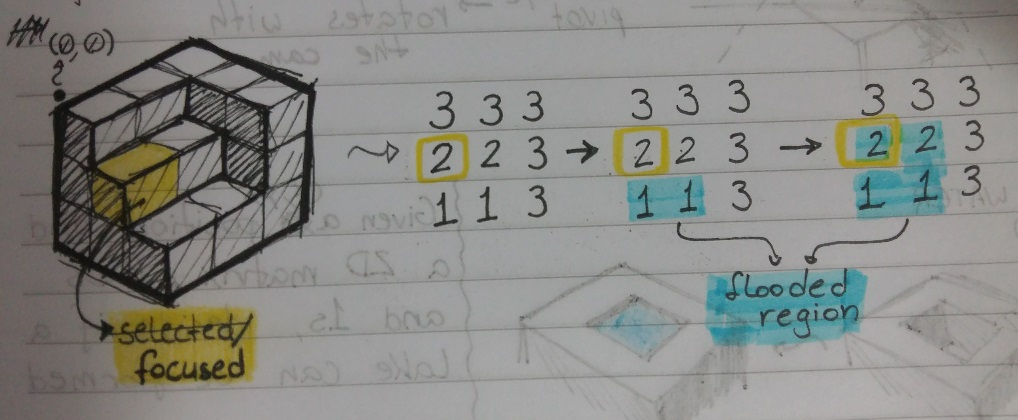
\includegraphics[width=0.5\textwidth]{water_mechanics2}
	\caption{Mecânicas da água 2}
\end{figure}

Nesta iteração, haveria dois gestos que deveriam ser captados e interpretados pelo Leap Motion: abaixar e elevar a mão com a palma aberta para alterar a elevação do terreno e apontar todos os dedos para baixo para fazer chover em uma área específica.

\begin{figure}[ht]
	\centering
	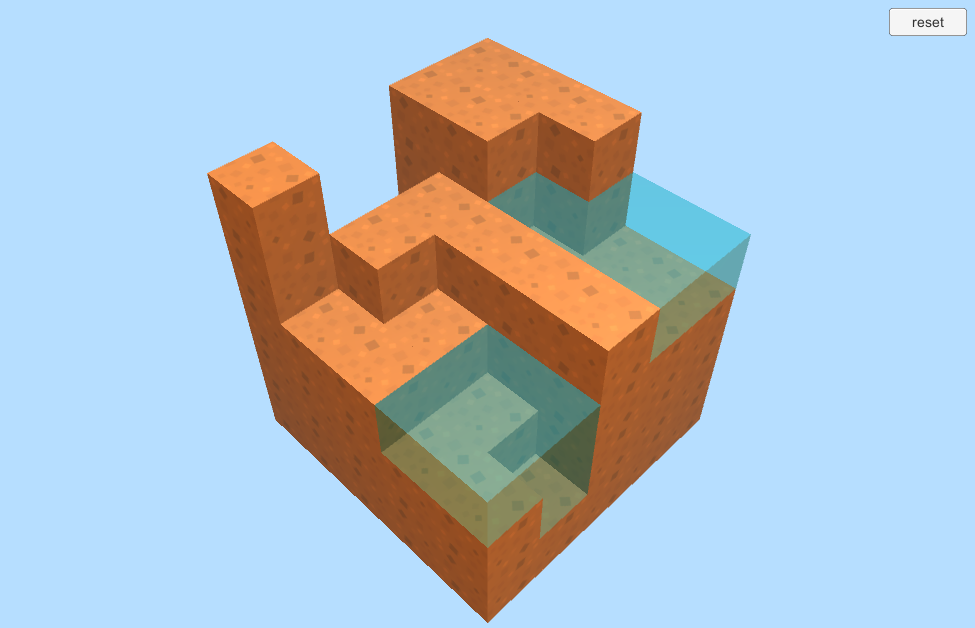
\includegraphics[width=0.5\textwidth]{ss2}
	\caption{Prova de conceito do jogo}
\end{figure}

Durante a implementação dessas mecânicas, ficou clara a necessidade de uma mecânica de seleção que permitisse a manipulação de grandes áreas do terreno simultaneamente, então um terceiro gesto foi adicionado: pinçar e arrastar para delimitar áreas.

Também nessa etapa, percebeu-se que, devido à posição do Leap Motion, alguns dos gestos imaginados para as diferentes mecânicas do jogo - sobretudo o associado a chuva - não poderiam ser captados com a precisão necessária, nos levando a precisar reimaginar uma parte significativa da interação.


% ---
\section{Arquitetura}\label{sec-desenvolvimento-arquitetura}
% ---

Para se definir a arquitetura do sistema, é antes necessário identificar e entender cada um dos principais elementos, assim como suas interfaces.

% ---
\subsection{Identificação dos elementos}\label{subsec-identificacao-elementos}
% ---

% ---
\subsubsection{Controlador Leap Motion}\label{subsubsec-elemento-leapmotion}
% ---

Conforme visto em \ref{subsubsec-teo-leap-motion}, o controlador pode ser dividido em 2 elementos diferentes: O \textbf{hardware do controlador} e o \textbf{serviço} que aplica algoritmos de visão computacional nas imagens vindas do hardware, transformando-as em dados estruturados.

O serviço pode ser executado no computador ou, no caso de se utilizar a versão 2 do SDK do Leap Motion, no Android.

% ---
\subsubsection{Lógica do jogo}\label{subsubsec-elemento-logica-jogo}
% ---

Este é o elemento que age sobre o ambiente virtual a partir de dados de entrada do controlador e do movimento do \textit{headset} de realidade virtual. Este elemento estará implementado no Unity, e pode ser executado ou no computador ou no próprio celular.

% ---
\subsubsection{Processamento de saída do video}\label{subsubsec-elemento-video}
% ---

Este elemento é controlado pelo SDK do Google Cardboard, e cuida de toda a parte de gerar a visão estereoscópica necessária para a visão 3D, além de movimentar a visão do jogo de acordo com o movimento do \textit{headset} de realidade virtual. Este elemento pode ser executado ou no computador ou no próprio celular.

% ---
\subsection{Arquiteturas estudadas}\label{subsec-arquiteturas-estudadas}
% ---

As três arquiteturas estudadas têm como entrada as imagens vindas do controlador Leap Motion e do movimento do Google Cardboard, que são enviadas à lógica de jogo que, então, modifica o estado do jogo e envia para o Google Cardboard. As diferentes opções de arquitetura diferem quanto à como a conexão é feita, se é intermediada ou não por um computador, e aonde essa intermediação acontece.

% ---
\subsubsection{Alternativa utilizando o servidor WebSocket}\label{subsubsec-arquiteturas-leapmotion-pc-leapdata-android}
% ---

Nesta opção, conecta-se o controlador a um computador que esteja rodando o serviço do Leap Motion, transformando as imagens do controlador em dados estruturados. Estes são, então, enviados a um celular que esteja rodando a lógica do jogo e fazendo as transformações necessárias para a saída de vídeo. Esta opção é demonstrada na figura \ref{fig:arquitetura-leap-pc-leapdata-android}.

As vantagens desta opção é que podemos utilizar a versão mais recente do SDK do Leap Motion, que melhorou muito o rastreamento das mãos, comparada à versão 2. Adicionalmente, o serviço já expõe uma interface web para a leitura dos dados estruturados. 

Uma desvantagen desta opção, porém, é a necessidade de modificar a biblioteca do Leap Motion do Unity para que esta aceite conexões web, já que, nativamente, ela aceita apenas conexões via USB. Outra desvantagem é a latência adicionada entre o movimento das mãos do usuário e o momento em que a lógica do jogo recebe tais informações. Se esta latência for alta demais, cria-se uma dissociação entre a mão do jogador e a mão virtual, diminuindo a imersão no jogo.

\begin{figure}
	\centering
	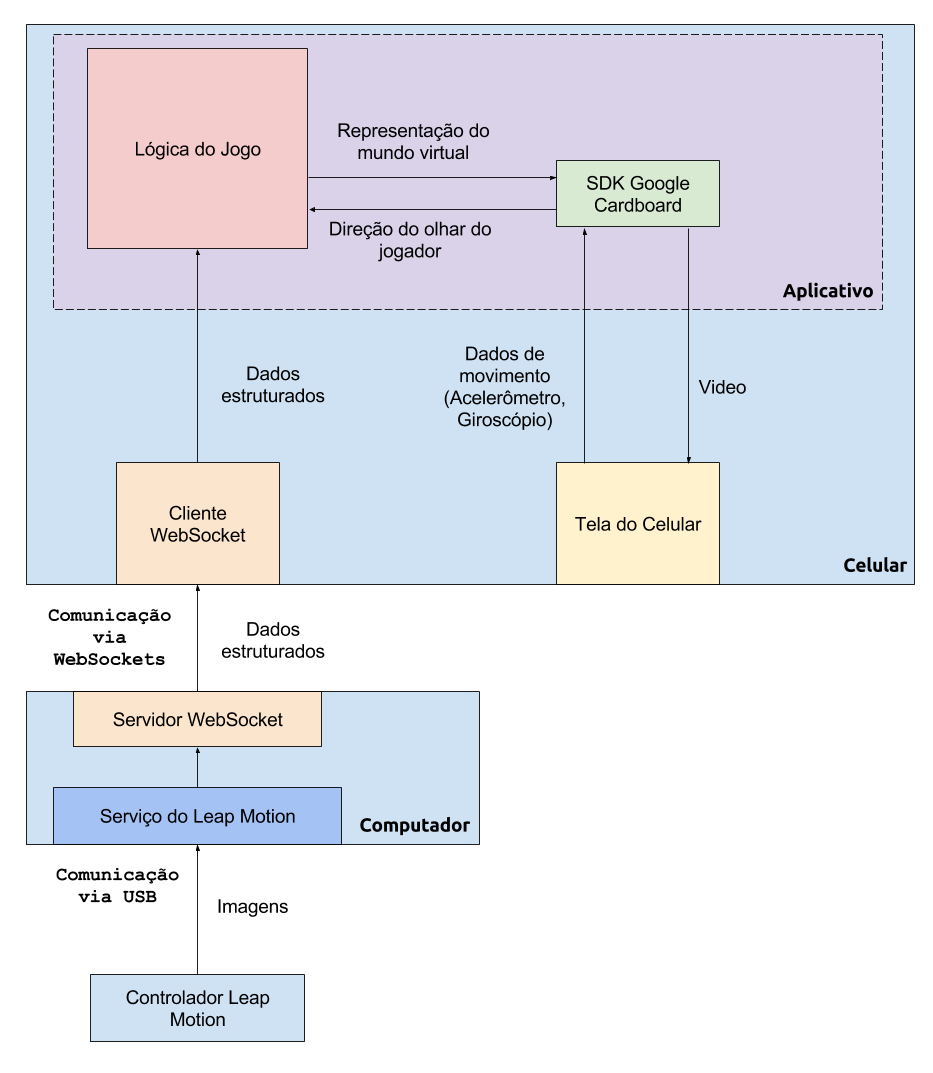
\includegraphics[width=0.7\linewidth]{images/Arquitetura-leap-pc-leapdata-android}
	\caption{Alternativa de arquitetura com servidor WebSocket}
	\label{fig:arquitetura-leap-pc-leapdata-android}
\end{figure}

% ---
\subsubsection{Alternativa com streaming do video}\label{subsubsec-arquiteturas-leapmotion-pc-riftcat-android}
% ---

O diferencial desta opção é que a lógica do jogo roda no computador, e a saída de vídeo é transmitida para o celular via algum software, como o Riftcat(pago) ou o TrinusVR(gratuíto). Desta forma, o controlador é conectado diretamente ao computador, que está rodando o serviço do Leap Motion e lê diretamente dele os dados estruturados.

As vantagens desta opção são que, por rodar num computador, o poder de processamento é mais alto e, portanto, existem mais possibilidades quanto a algoritmos utilizados, mecânicas do jogo e processamento gráfico. A conexão com o controlador, por ser direta, também significa uma latência baixa. 

O principal contraponto desta opção é o aumento da latência entre o movimento da cabeça do usuário e o movimento da cabeça virtual. Esta latência é maior do que a da opção 1 pois é necessário enviar os dados referentes ao movimento da cabeça do celular para o computador, que então deve enviar as imagens de volta para o celular. Essa latência adicional não apenas cria uma dissociação entre o jogador e o mundo virtual, mas também pode causar tontura e enjoo.

\begin{figure}
	\centering
	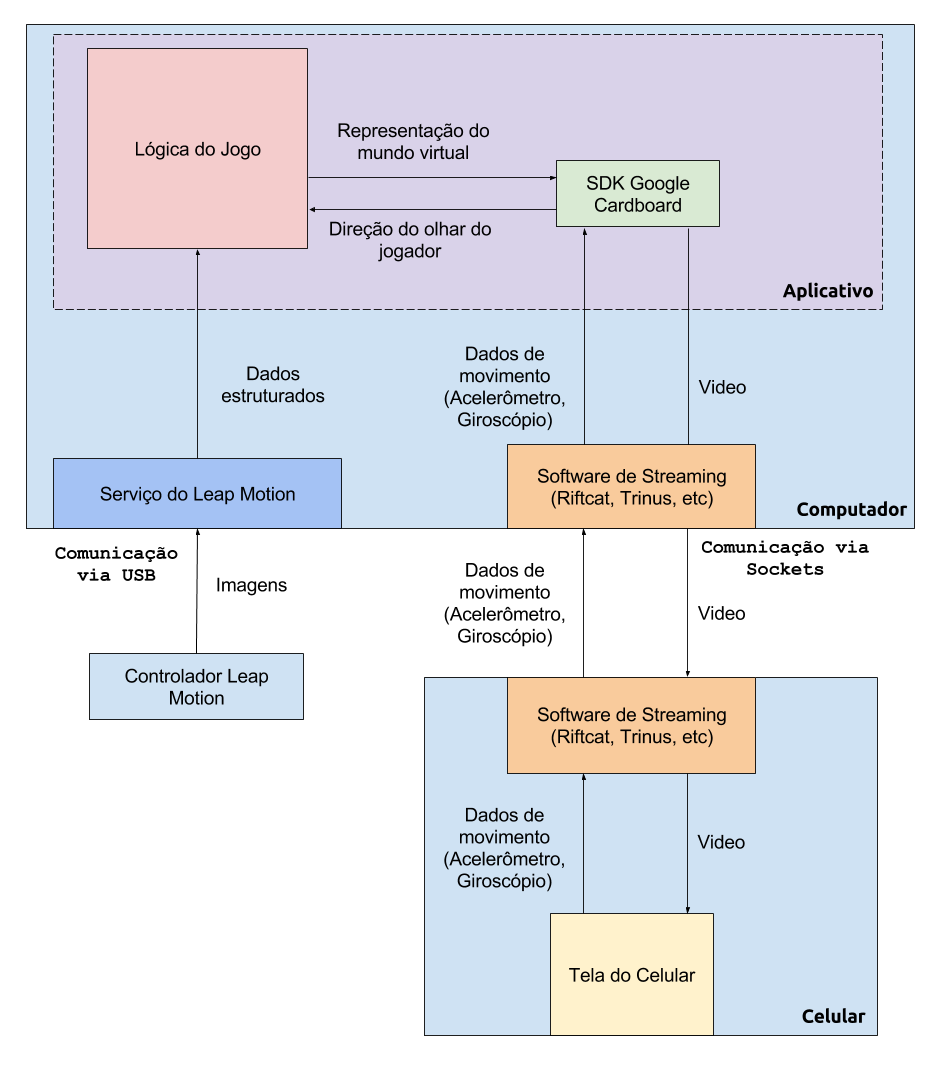
\includegraphics[width=0.7\linewidth]{images/Arquitetura-leap-pc-riftcat-android}
	\caption{Alternativa de arquitetura com streaming do video}
	\label{fig:Arquitetura-leap-pc-riftcat-android}
\end{figure}

% ---
\subsubsection{Alternativa com conexão direta}\label{subsubsec-arquiteturas-leapmotion-android}
% ---

Nesta opção, o controlador é conectado diretamente ao celular, conforme mostrado na figura \ref{fig:arquitetura-leap-android}. Desta forma, esta opção provê a maior mobilidade e tem o menor número de subsistemas diferente. Para tal, é necessário utilizar o serviço do Leap Motion v2 específica para o Android. Neste caso, todo o processamento é feito diretamente no celular: A transformação das imagens em dados estruturados, a lógica do jogo e as transformações necessárias para a saída de video. Por esta razão, esta é a opção que adiciona a menor latência, devido à inexistência de conexões extras entre um computador e o celular, como nas outras opções.

As desvantagens, porém, são a dependência do serviço do Leap nativo do Android, que estava na versão beta antes de ser descontinuado, e também o fato de se tratar da versão 2, que tem um rastreamento pior.

\begin{figure}
	\centering
	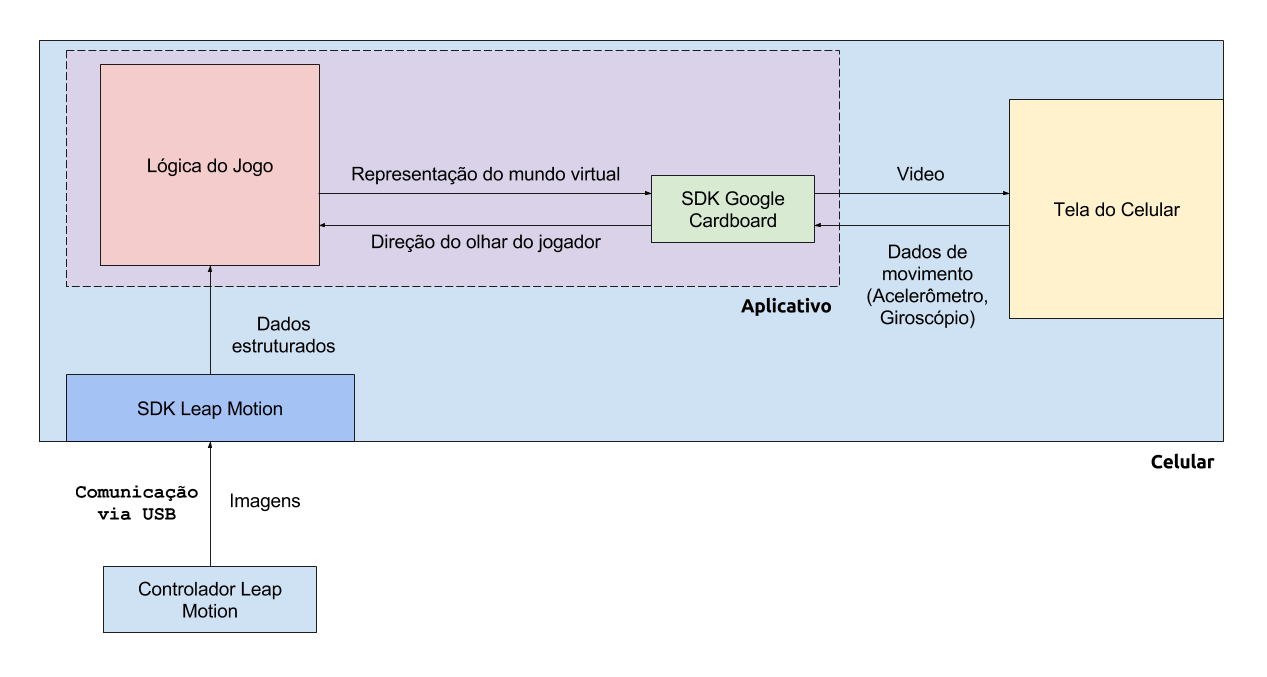
\includegraphics[width=0.7\linewidth]{images/Arquitetura-leap-android}
	\caption{Alternativa de arquitetura com conexão direta}
	\label{fig:arquitetura-leap-android}
\end{figure}

% ---
\subsubsection{Comparação das alternativas}\label{subsubsec-arquiteturas-comparacao}
% ---

A comparação das alternativas pode ser vista na tabela \ref{tabela:alternativas-arquiteturas}.

\begin{table}[!h] \scriptsize
	\centering
	\begin{tabular}{|>{\centering\arraybackslash}m{2.1cm}|>{\centering\arraybackslash}m{6cm}|>{\centering\arraybackslash}m{6cm}|}
		\hline 
		\textbf{Alternativa} & \textbf{Pros} & \textbf{Contras} \\
		\hline 
		Servidor Websocket
		&\begin{itemize}[label={--},noitemsep,topsep=0pt,leftmargin=4mm]
			\item Versão mais recente do SDK do Leap.
			\item Servidor WebSocket já disponível com o serviço Leap Motion.
		\end{itemize}
		&\begin{itemize}[label={--},noitemsep,topsep=1pt,leftmargin=4mm]
			\item Maior latência entre o movimento da mão e da mão do jogador, pode diminuir imersão.
			\item Necessidade de modificação da biblioteca do Leap no Unity.
		\end{itemize}
		\\ \hline 
		Streaming de Video
		&\begin{itemize}[label={--},noitemsep,topsep=0pt,leftmargin=4mm]
			\item Processamento feito no computador
			\item Conexão direta da lógica do jogo com controlador
		\end{itemize}
		&\begin{itemize}[label={--},noitemsep,topsep=0pt,leftmargin=4mm]
			\item Latência entre movimento da cabeça do jogador e movimento da cabeça virtual, podendo causar desconforto e náusea.
			\item Dependência de mais software, podendo ser pago.
		\end{itemize}
	    \\ \hline 
		Conexão Direta
		&\begin{itemize}[label={--},noitemsep,topsep=0pt,leftmargin=4mm]
				\item Menor latência dentre as opções
			\end{itemize}
		&\begin{itemize}[label={--},noitemsep,topsep=0pt,leftmargin=4mm]
				\item Utiliza a versão v2 do SDK do Leap, que tem precisão pior.
				\item Necessita da versão beta do serviço para o Android, de difícil acesso.
			\end{itemize}
		\\ 
		\hline 
	\end{tabular} 
	\caption[Comparação das alternativas de arquitetura]{Comparação das alternativas de arquitetura}
\label{tabela:alternativas-arquiteturas}
\end{table}

% ---
\subsection{Escolha da arquitetura}\label{subsec-arquitetura-escolha}
% ---

Inicialmente, se optou pela alternativa do streaming de video, visto que a sua implementação não necessitaria de mudanças no código. Bastaria gerar o executável do jogo no windows e rodar um software de streaming, como o Riftcat. Durante o desenvolvimento inicial, esta foi a alternativa utilizada, mesmo sendo necessário inicializar o software várias vezes, devido a bugs e falta de documentação do Rifcat.

Porém, descobriu-se posteriormente que para que esta alternativa funcionasse, era necessário uma placa de video relativamente potente, de acordo com as especificações mínimas do software, encontrada em \cite{riftcat:2016:requirements}. Inclusive, o software do Riftcat só funcionava em um dos 5 computadores testados. Por esta razão, optou-se por abandonar esta alternativa, visto que dificultaria a acessibilidade do jogo.

Dado este contratempo, decidiu-se testar as outras duas alternativas para verificar suas viabilidades. 

A alternativa da conexão direta necessitava a obtenção da versão do serviço do Leap Motion para o Android, que não estava mais disponível no website da empresa. Afortunadamente, a co-orientadora deste projeto havia trabalhado anteriormente com o Leap Motion no Android, e conseguiu uma cópia dos arquivos necessários. Entretanto, nos testes preliminares feitos, não se obteve sucesso na utilização do serviço: O aplicativo do software no celular reconhecia o controlador conectado, mas aplicativos 'clientes' que utilizariam os dados do controlador não conseguiam se conectar ao controlador. Por este motivo, esta alternativa foi descartada.

Optou-se então pela alternativa que restou, que utiliza o servidor WebSocket gerado pelo serviço do Leap Motion no computador. A principal dificuldade desta alternativa é que o plugin disponibilizado pela empresa para o Unity só conseguia receber os dados do controlador por meio da conexão direta, e não pelo servidor WebSocket. Portanto, foi necessário modificar o plugin distrubuído, que é software livre e tem seu código fonte disponível, para que ele se conectasse ao servidor WebSocket, recebesse os dados estruturados em mensagens JSON, parseasse-as e então as transformasse na estrutura de dados utilizada pelo Unity.

Para implementar tais mudanças no código do plugin, foi necessário encontrar e testar bibliotecas que se conectassem a um servidor WebSocket (visto que o Unity não consegue fazer isto nativamente) e parseasse JSON (pois o \textit{parser} JSON nativo do Unity só funciona em casos de uso muito limitados). Visto que é necessário que movimentos das mãos sejam refletidos o mais rapidamente o possível no jogo (para se manter a impressão de que as mãos virtuais são as mãos reais do usuário, para manter a imersão), é essencial que estas bibliotecas fossem rápidas o suficiente para não serem um gargalo, além de serem eficientes em questão de memória e objetos alocados, visto que rodam com frequencia alta e é o Unity que gere a sua memória (ou seja, o Unity roda o coletor de lixo de tempos em tempos, algo que pode causar travamentos dependendo de quantos objetos 'mortos' existirem).

